\chapter{Einleitung}

Durch die fortschreitende Miniaturisierung der Technik enstand im 20. Jahrhundert
die Notwendigkeit Strukturen abzubilden, die kleiner waren als die Wellenlänge des
Lichts. Herkömmliche optische Mikroskope boten in diesem neuen Bereich, der 
Nanowissenschaft, nicht mehr die notwendige Genauigkeit. Ein wichtiger Schritt
gelang den Physikern Gerd Binning und Heinrich Rohrer 1981, als sie mit dem 
experimentellen Nachweis eines abstandabhängigen Tunnelstroms den Grundstein für
das Rastertunnelmikroskop legten.\\
Aus dieser Erfindung ist seither eine ganze Familie an Rastersondenmikroskopen
hervorgegangen, die sich unterschiedliche Wechselwirkungen auf automarer Skala
zu nutze machen. Das bekannste ist wohl das Rasterkraftmikroskop, welches die 
Kräfte zwischen der Materialoberfläche und der Messspitze messen kann. Weiter
wurden das optische Rasternahfeldmikroskop und das Magnetkraftmikroskop entwickelt.
Erst die Entwicklung dieser Mikroskopfamilie hat die Beobachtung und Manipulation
von Nanostrukturen einfach und preiswert genug für den weitläufigen Einsatz in 
Unternehmen gemacht.\\
Dies hat wesentlich zur Veranschaulichung der Quantenmechanik beigetragen.
\begin{wrapfigure}{r}{0.3\textwidth}
    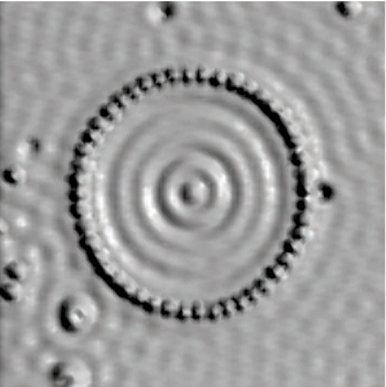
\includegraphics[scale=1.25]{Abb/quant.jpg}
    \caption{Quantum Corral \cite{corral}}
    \label{qucorr}
\end{wrapfigure}
Ein Beispiel bieten hier die "Quantum Corrals", wie in Abbildung \ref{qucorr} zu
sehen. Hierbei handelt es sich um einfache Quantensysteme Oberflächen. In obigem
Beispiel sind Goldatome radial auf einer Kupferoberfläche angeordnet. Anschaulich
gezeigt werden hier die Elektronenwellen im Inneren der Anordnung.
Derartige Messungen erreichten schnell große Beliebtheit und sind in 
populärwissenschaftlichen Zeitschriften häufig Thema. 
\cite{rasterwiki}
% 
